\documentclass[border=10pt]{standalone}
\usepackage{amsmath}
\usepackage{tikz}
\usetikzlibrary{arrows.meta}
\definecolor{acc}{HTML}{0D9488}
\definecolor{ink}{HTML}{1A1D21}
\definecolor{mut}{HTML}{646A72}
\newcommand{\tok}[3]{%
  \edef\tokval{#3}\def\blank{-}\ifx\tokval\blank\node[draw=mut, fill=mut!10, text=mut, minimum size=5.4mm, inner sep=0, font=\small] at (#1,#2) {$\epsilon$};%
  \else\node[draw=ink, fill=acc!12, text=ink, minimum size=5.4mm, inner sep=0, font=\small\ttfamily\bfseries] at (#1,#2) {#3};\fi}
\newcommand{\row}[3]{\foreach \c [count=\i from 0] in #3 {\tok{#1+0.6*\i}{#2}{\c}}}
\begin{document}
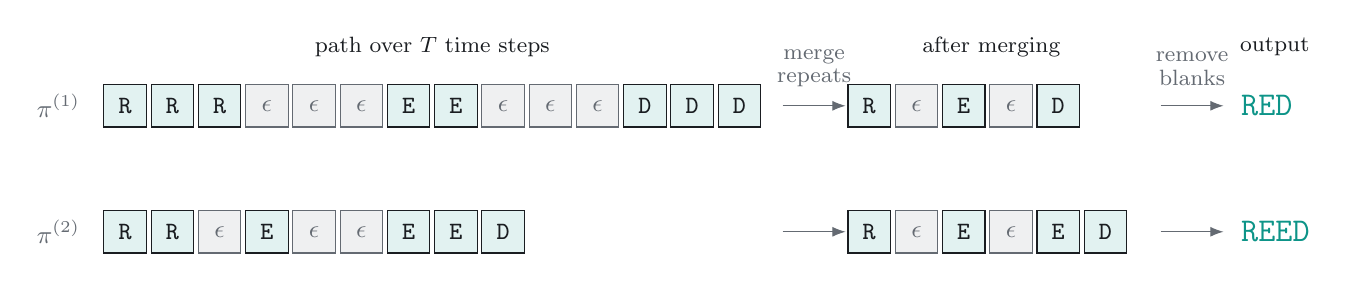
\begin{tikzpicture}[>=Latex, font=\small]
  \foreach \y/\pth/\mrg/\out/\nm in {
      0/{R,R,R,-,-,-,E,E,-,-,-,D,D,D}/{R,-,E,-,D}/RED/{\pi^{(1)}},
      -1.6/{R,R,-,E,-,-,E,E,D}/{R,-,E,-,E,D}/REED/{\pi^{(2)}}} {
    \node[anchor=east, text=mut] at (-0.45,\y) {$\nm$};
    \row{0}{\y}{\pth}
    \draw[->, mut] (8.35,\y) -- (9.15,\y);
    \row{9.45}{\y}{\mrg}
    \draw[->, mut] (13.15,\y) -- (13.95,\y);
    \node[anchor=west, font=\large\ttfamily\bfseries, text=acc] at (14.05,\y) {\out};
  }
  \node[text=mut, font=\footnotesize] at (8.75,0.62) {merge};
  \node[text=mut, font=\footnotesize] at (8.75,0.35) {repeats};
  \node[text=mut, font=\footnotesize] at (13.55,0.62) {remove};
  \node[text=mut, font=\footnotesize] at (13.55,0.35) {blanks};
  \node[text=ink, font=\footnotesize] at (3.9,0.75) {path over $T$ time steps};
  \node[text=ink, font=\footnotesize] at (11.0,0.75) {after merging};
  \node[text=ink, font=\footnotesize] at (14.6,0.75) {output};
\end{tikzpicture}
\end{document}
